\subsection{Node.js}
\label{sec:nodejs}
Node.js (anche conosciuto come Node o Nodejs) è un framework/piattaforma molto potente basato sul motore \textit{JavaScript V8} di Google Chrome, per creare facilmente applicazioni di Web veloci e scalabili. Pubblicata da Ryan Dahl nel 2009, viene utilizzato per sviluppare applicazioni Web intensive di I/O come siti di streaming video, applicazioni a pagina singola e altre applicazioni Web. Node.js è un ambiente open source, multi-piattaforma per lo sviluppo di applicazioni lato server completamente gratuito, utilizzato da migliaia di sviluppatori in tutto il mondo. Le applicazioni Node.js sono scritte in Javascript e possono essere eseguite all'interno del runtime di Node.js su OSX, Microsoft Windows e Linux. 
\\Utilizza un modello I/O non bloccante e basato sugli eventi che lo rende leggero ed efficiente, perfetto per applicazioni in tempo reale ad alta intensità di dati che funzionano su dispositivi distribuiti \cite{node:home}. Il modello di networking su cui si basa Node.js non è quello dei processi concorrenti, ma I/O event-driven: ciò vuol dire che Node richiede al sistema operativo di ricevere notifiche al verificarsi di determinati eventi, e rimane quindi in sleep fino alla notifica stessa: solo in tale momento torna attivo per eseguire le istruzioni previste nella funzione di \textit{callback}, così chiamata perché da eseguire una volta ricevuta la notifica che il risultato dell'elaborazione del sistema operativo è disponibile. Tale modello di networking, implementato anche nella libreria Event machine per Ruby e nel framework Twisted per Python, è ritenuto più efficiente nelle situazioni critiche in cui si verifica un elevato traffico di rete \cite{node:wiki}. In definitiva, di fronte alle esigenze di migliorare le performance dei software di rete Ryan Dahl ha creato una piattaforma in che esegue le operazioni di I/O particolarmente lente (comunicazioni di rete o accesso al disco) in modo asincrono, rendendo la programmazione su Node JS diversa da qualsiasi esperienza con altri linguaggi. In definitiva, l'obiettivo di Node.js è quello di fornire un modo veloce per realizzare applicazioni web scalabili in termini di gestione delle connessioni da parte dei client verso il web server.
\\Node.js nel momento in cui una operazione di I/O considerata lenta (di solito lo è se riguarda la rete o il disco fisso) viene eseguita da un programma in Node JS, V8 si occupa di trasferire la chiamata su un thread non bloccante fra quelli che ha a disposizione nella sua thread-pool base. In questo modo, il thread principale con il codice può continuare la sua esecuzione senza context switch. Nel momento in cui una operazione collegata ai thread non bloccanti è terminata il kernel segnala che questo thread può tornare in coda di esecuzione. A questo punto però V8 si occuperà di intercettare il messaggio, mettere nella propria coda di esecuzione la funzione di callback specificata con l'operazione di I/O terminata e di rimettere il thread non bloccante a disposizione per altre operazioni di I/O. Così facendo, virtualmente il thread che esegue codice non si ferma mai, avvicendando le funzioni di callback delle varie operazioni terminate [\ref{fig:nodeEvent}].
\begin{figure}[H]
	\centering
	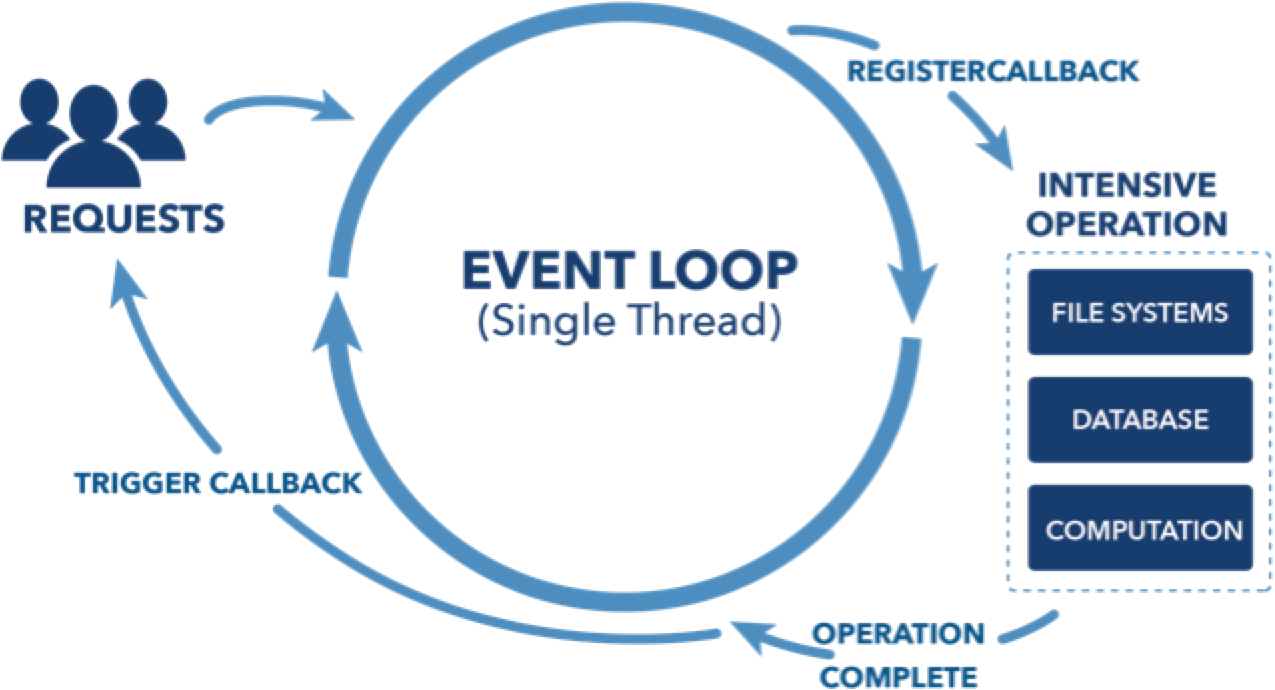
\includegraphics[width=\textwidth]{images/nodeEvent.png}
	\caption{Gestione eventi con Node.js.}
	\label{fig:nodeEvent}
\end{figure}
Bisogna però sempre tenere a mente, quando si progetta di scrivere un programma con Node.js, che questa architettura ha un effetto collaterale molto pesante; le operazioni che occupano per lungo tempo il thread in cui viene eseguito il codice (operazioni di calcolo onerose) bloccano l'interno software. Per questo motivo Node.js è assolutamente sconsigliato in caso di operazioni di calcolo complesse e nella fase di progettazione di programmi che usano questa piattaforma è sempre necessario utilizzare questa caratteristica come criterio fondamentale per la scrittura del codice.
Di seguito sono alcune delle caratteristiche importanti che rendono Node.js la prima scelta di architetti del software:
\begin{itemize}
\item \textbf{Asynchronous and Event Driven}: Tutte le API della libreria Node.js sono asincrone, ovvero non bloccanti. Significa essenzialmente che un server basato su Node non aspetta mai che un'API restituisca i dati. Il server passa all'API successiva dopo averlo chiamato ed un meccanismo di notifica di eventi consente al server di ottenere una risposta dalla precedente chiamata.
\item \textbf{Molto veloce}: Essendo costruito sul motore Javascript V8 di Google Chrome, Node.js è molto veloce nell'esecuzione del codice.
\item \textbf{Thread singolo ma altamente scalabile}: Node utilizza un singolo thread con loop di eventi. Il meccanismo degli eventi aiuta il server a rispondere in modo non bloccante e rende il server altamente scalabile rispoetto ai server tradizionali che creano thread limitati per gestire le richieste. Quindi, Node utilizza un singolo programma con thread e lo stesso programma può fornire il servizio a un numero molto più grande di richieste rispotto ai server come Apache HTTP Server.
\item \textbf{Nessun Buffering}: Le applicazioni create con node non bufferizzano mai alcun dato. Queste applicazioni generano semplicemente i dati in blocchi.
\item \textbf{Licenza}: Node è rilasciato sotto licenza MIT. 
\end{itemize}
Esiste un mondo attorno a JS composto da librerie che ne estendono le funzionalità. Stesso discorso vale per Node.js, in quanto è attiva una comunità di sviluppo che ha realizzato in questi anni molte librerie per realizzare particolari tipi di supporto (database, Network, . . . ) e Node.js offre un sistema di installazione di questi moduli che si occupa anche di eventuali dipendenze: \textit{npm}. Nei prossimi capitoli saranno analizzati alcuni progetti legati a Node.js usati nella creazione della webapp.

\subsubsection{Express.js ed Handlebars}
\label{sec:express handlebars}
Express.js (anche chiamato semplicemente Express) è un framework basato su Node.js che offre un insieme robusto di utilità per realizzare agilmente un'architettura \textit{MVC (Model-View-Controller)} sul lato server di applicazioni web single-page, multi-page ed ibride.
\\Basato sul modulo di Node chiamato \textit{connect}, risulta essere un ottimo "connettore" o \textit{middleware} tra le diverse librerie che possono popolare una webapp, tra cui WebSocket, Passport, Mustache.js, Handlebars, etc.
\\Le funzionalità offerte sono il \textit{routing}, la possibilità di gestire le configurazioni dell'applicazione ed un motore di templating.
\\Al centro di questa libreria c'è il concetto di flusso di funzioni, o come piace dire a certe persone, un set di \textit{livelli di funzione}. Infatti, per creare un'applicazione Express c'è bisogno di creare una sequenza di funzioni (livelli) che il framework può navigare. 
\\Quando una di queste decide di entrare in gioco, può completare il processo e fermare la sequenza. Dopodiché Express riprende a scorrere la sequenza fino alla fine.
\\Queste funzioni hanno delle callback associate che sono eseguite nel momento in cui un client effettua una richiesta. Questo processo prende il nome di Routing.
\\Il routing, dunque, è una funzionalità di Express.js, che determina la risposta ad una richiesta client ad un endpoint particolare; il quale può essere un URI (o percorso) o un metodo di richiesta HTTP specifico. In pratica, con Express, si possono gestire le richieste e le risposte \textit{in the middle}, cioè fra server e client. Quando il server riceve una richiesta HTTP la racchiude all'interno di un oggetto \textit{ServerRequest}. Questo oggetto, insieme all'oggetto \textit{ServerResponse}, viene passato al primo middleware che ne può modificare il contenuto, o aggiungere proprietà. Una volta terminata la modifica, il middleware richiamerà il successivo nell'eventuale catena (di funzioni) presente.
\begin{figure}[H]
	\centering
	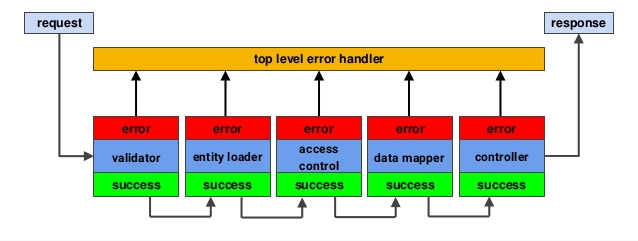
\includegraphics[width=\textwidth]{images/ExpressRoute.png}
	\caption{Visualizzazione della catena di funzioni per rispondere ad una richiesta}
	\label{fig:expressFlow}
\end{figure}
Se l'ultima funzione della catena deve restituire un HTML come risultato, Express chiama in causa il \textit{template engine}. Questo motore, infatti si occupa di fare il tramite tra i dati presenti nel layer model e quello di presentazione. In particolare elabora la richiesta producendo, in fase di run-time, un HTML dinamico partendo da una struttura definita (template). Esistono diversi motori che possono essere utilizzati con Express ognuno con le proprie particolarità e specifiche. 
\\Per questo elaborato la scelta del templating engine è caduta su \textit{Handlebars.js}. La libreria di templating Handlebars consente di creare un'interfaccia utente ricca includendo HTML statico e contenuto dinamico, che possono essere specificati nelle doppie parentesi graffe. Handlebars.js è molto popolare, semplice da usare e con una grande community. È basato sul linguaggio dei modelli di Mustache, ma lo migliora in molti aspetti. Con Handlebars, si può separare la generazione di HTML dal resto del JavaScript e scrivere codice più pulito. Inoltre, aggiunge costrutti (if e cicli for) che permettono di creare dinamicamente l'HTML. Infine, introduce un sistema di \textit{partial} che permette allo sviluppatore di inserire nelle proprie pagine, porzioni di HTML provenienti da file esterni. 
\\Express, quindi, per costruire la pagina di risposta da inviare al client, chiama Handlerbars che preleva i file con estensione \textit{.handlebars} li "compila" e genera il risultato finale.

\begin{lstlisting}[language=HTML, label=lst:HandlebarsTemplate, caption={Esempio di HTML scritto con Handlebars.}]
<div class="entry">
  <h1>{{title}}</h1>
  <h2>By {{author.name}}</h2>
  <div class="body">
    {{body}}
  </div>
</div>
\end{lstlisting} 

Il listato \ref{lst:HandlebarsTemplate} è un esempio di HTML scritto con la sintassi di Hadelbars. I valori \textit{title}, \textit{author.name} e \textit{body} saranno sostituiti, in fase di run-time, con i valori provenienti dal controller che passerà un oggetto all'engine templating. vedi listato \ref{lst:handleCode}.

\begin{lstlisting}[language=Javascript, label=lst:handleCode, caption={Esempio di variabile passata dal controller al template engine.}]
var context = {
  title: "My First Blog Post!",
  author: {
    id: 47,
    name: "Yehuda Katz"
  },
  body: "My first post. Wheeeee!"
};
\end{lstlisting} 

\subsubsection{WebSocket}
\label{sec:WebSocket}

\subsubsection{MaterialCSS}
\label{sec:materialCSS}

\subsubsection{D3js}
\label{sec:d3js}